\documentclass[10pt,a4paper]{article}
\usepackage{ngerman}
\usepackage{enumitem, fancyhdr, graphicx, lastpage, sectsty, xcolor}
\usepackage[hidelinks]{hyperref}
%\usepackage{authblk}

\definecolor{dunkelblau}{rgb}{0.2,0.2,0.8}
\subsectionfont{\color{dunkelblau}}

\title{ISF HS 2019}
\author{Victor Fernández\\Pavaskar Parameswaran}
\date{Dezember 2019}


\addtolength{\oddsidemargin}{-.875in}
\addtolength{\evensidemargin}{-.875in}
\addtolength{\textwidth}{1.75in}
\addtolength{\topmargin}{-.875in}
\addtolength{\textheight}{1.75in}

% muss nach Änderung der margin kommen!
\pagestyle{fancy}
\fancyhf{} %reset
\fancyhead[L]{HSLU}
\fancyhead[C]{ISF}
\fancyhead[R]{\thepage/\pageref{LastPage}}
\fancyfoot[L]{}
\fancyfoot[C]{}
\fancyfoot[R]{}
\renewcommand{\headrulewidth}{0.2pt} % Strich in Kopfzeile

%******
\begin{document}
\maketitle
\thispagestyle{empty}
\section*{Vorwort}Diese Zusammenfassung entstand in einer Gruppe während der Lernphase des HS 2019. Alle Fragen aus der Stoffabgrenzung tragen eine {\color{dunkelblau}blaue Farbe} und stehen als Unterkapitel. Das Dokument ist Open Source und jeder der möchte und signifikant beiträgt, darf sich als Autor anhängen. Die Source ist \underline{\href{https://github.com/vigi86/HSLU_Zusammenfassungen/tree/master/ISF_HS19}{dieses GitHub-Repo}}. Dies ist mein erstes \LaTeX{}-Dokument überhaupt. Nichts desto trotz wurde auf eine klare Strukturierung und Lesbarkeit des Dokumentes Wert gelegt.
\tableofcontents
\thispagestyle{empty}
\pagebreak

\part{Einführung (SW~01)}
\section{Einführung}
\subsection*{Einführung in das Thema "`Management von Informationssicherheit"'}
\paragraph*{Daten, Information und Wissen}
Information ist die Verknüpfung von Daten in Form von Zahlen, Worten und Fakten zu interpretierbaren Zusammenhängen.
Durch die Vernetzung von Informationen entsteht Wissen, das zunächst personenbezogen ist.
\paragraph*{Missbrauch}Informationen müssen vor Missbrauch geschützt werden
\begin{figure}[ht]
    \begin{center}
    \includegraphics[width=8cm]{images/Wissenspyramide.png}
    \caption{Wissenspyramide}
    \label{Wissenspyramide}
    \end{center}
\end{figure}


\subsection*{Motivation / Bedrohungen}
\paragraph*{Was gefährdet die Informationen?} Welche Gefährdungen/Bedrohungen gibt es?
\begin{itemize}[noitemsep,topsep=0pt,leftmargin=*]
    \item Nicht vorsätzliche (zufällige) Gefährdungen/Bedrohungen
    \begin{itemize}[noitemsep,topsep=0pt,leftmargin=*]
        \item Naturgewalten (Blitz, Hagel, Unwetter, Erdrutsche, Hochwasser, etc.)
        \item Ausfall von Strom oder Telekommunikation
        \item Technische Pannen, z.B. Fehler von Hard- und/oder Software
        \item Bedienerfehler / Fahrlässigkeit der Mitarbeitenden
    \end{itemize}
    \item Vorsätzliche Gefährdungen/Bedrohungen
    \begin{itemize}[noitemsep,topsep=0pt,leftmargin=*]
        \item Bösartiger Code (Viren, Würmer, Trojaner, etc.)
        \item Informationsdiebstahl
        \item Angriffe (von Skript-Kiddies bis Hacker)
        \item Wirtschaftsspionage ("`was die Konkurrenz wissen möchte"')
        \item Missbrauch der IT-Infrastruktur
    \end{itemize}
\end{itemize}

\subsection*{Grundbegriffe}
\textbf{Zutritts-, Zugangs-, Zugriffskontrolle}
\begin{itemize}[noitemsep,topsep=0pt,leftmargin=*]
    \item \textbf{\textsl{Zutrittskontrolle: }}Schutz des physischen Systems (Bsp. Serverraum)
    \item \textbf{\textsl{Zugangskontrolle: }}Schutz des logischen Systems (Bsp. Betriebssystem)
    \item \textbf{\textsl{Zugriffskontrolle: }}Daten-bezogen; Schutz der Operationen (Bsp. Dateisystem)
\end{itemize}


\part{Kryptographie (SW~02-04)}
\section{Symmetrische Kryptographie}
\subsection*{Sie verstehen was Steganographie ist}
\paragraph*{TODO}
\subsection*{Sie verstehen was Private-Key-Kryptographie ist, welche Arten von Sicherheit es gibt und welche Angriffsarten auf Verschlüsselung existieren}
\paragraph*{TODO}
\subsection*{Sie können "`klassische"' symmetrische Verschlüsselungverfahren wie Ceasar cipher, Vigenère cipher, one-time pad anwenden und verstehen die Vor- und Nachteile bzw. Schwachstellen dieser Verfahren}
\paragraph*{TODO}
\subsection*{Sie wissen welche modernen Verschlüsselungsalgorithmen in der Praxis verwendet werden und was deren Eigenschaften sind}
\paragraph*{TODO}
\subsection*{Sie verstehen was eine Hashfunktion ist und welche Eigenschaften eine kryptographische Hashfunktion ausmachen, bzw. was es heisst, wenn eine Hashfunktion gebrochen ist}
\paragraph*{TODO}
\subsection*{Sie kennen moderne Hashfunktionen und wissen welche Eigenschaften diese haben}
\paragraph*{TODO}
\subsection*{Sie kennen Anwendungen von Hashfunktionen}
\paragraph*{TODO}
\subsection*{Sie wissen was ein keyed Hash (HMAC) ist und wofür dieser verwendet werden kann}
\paragraph*{TODO}
\subsection*{Sie kennen die "`Best-practices"' zu Passwortsicherheit und wissen, gegen welche Angriffe diese schützen}
\paragraph*{TODO}


\section{Asymmetrische Kryptographie}
\subsection*{Sie verstehen was Public-Key-Kryptographie ist, worauf deren Sicherheit basiert und wie sie zur Verschlüsselung, für Signaturen und zur Authentisierung verwendet werden kann}
\paragraph*{TODO}
\subsection*{Sie kennen die gängigen asymmetrischen Verschlüsselungs- und Signaturalgorithmen und wissen, worauf deren Sicherheit basiert}
\paragraph*{TODO}
\subsection*{Sie wissen wie Diffie-Hellmann-Schlüsselaustausch bzw. ElGamal-Verschlüsselung funktioniert}
\paragraph*{TODO}
\subsection*{Sie wissen was kryptographisch sichere Zufallszahlen sind und wo diese verwendet werden}
\paragraph*{TODO}
\subsection*{Sie wissen was eine elektronische Signatur ausmacht}
\paragraph*{TODO}
\subsection*{Sie wissen wie hybride Verschlüsselung bzw hybride Signaturen funktionieren}
\paragraph*{TODO}


\section{Zertifikate und SSL-TLS}
\subsection*{Sie kennen die verschiedenen Arten von "`Trust"'}
\paragraph*{TODO}
\subsection*{Sie wissen was eine Public-Key-Infrastruktur, eine Certificate Authority und ein Zertifikat ist, wofür und wie diese verwendet werden und wie Zertifikate ausgestellt und revoziert werden}
\paragraph*{TODO}
\subsection*{Sie wissen was SSL/TLS ist, welche Funktionalität es erreicht und wie das Protokoll konzeptionelle abläuft}
\paragraph*{TODO}



\part{Angriffe (SW~05-06)}
\section{Angriffe auf Webanwendungen}
\paragraph*{Bedrohungen auf Anwendungsebene}Webanwendung, Session, Headers, CSRF
\subsection*{Sie wissen was eine Webanwendung ausmacht, wie HTTP funktioniert}
Was unterscheidet eine Webanwendung aus Sicherheitssicht zu anderen Anwendungen?
\begin{itemize}[noitemsep,topsep=0pt,leftmargin=*]
    \item Kommuniziert über HTTP mit einem Server
    \begin{itemize}[noitemsep,topsep=0pt,leftmargin=*]
        \item zustandsloses Protokoll
    \end{itemize}
    \item Läuft in einem Browser
    \begin{itemize}[noitemsep,topsep=0pt,leftmargin=*]
        \item Mehrere Webanwendungen können parallel im gleichen Browser laufen
        \item Die Webanwendung \textsl{erbt} vom Browser implementierte Features
        bzw. muss diese richtig ansprechen
    \end{itemize}
\end{itemize}
\paragraph*{HTTP}Der Browser kommuniziert mit dem Webserver über das \textbf{Hypertext Transfer Protokoll (HTTP)}. HTTP besteht aus \textsl{Requests} und \textsl{Reponses}.
\paragraph*{HTTP-Request-Methoden}Die häufigsten HTTP-Request-Methoden sind \textbf{GET} und \textbf{POST}.
Es existieren aber auch \textbf{PUT, HEAD, DELETE, PATCH, OPTIONS}.
\paragraph*{GET} https://www.hslu.ch/?p=5 HTTP/1.1 User-Agent: Mozilla/5.0
\begin{itemize}[noitemsep,topsep=0pt,leftmargin=*]
    \item Message Body: kein
    \item Ruft Daten vom Server ab
    \item Sollte Serverzustand nicht verändern
\end{itemize}
\paragraph*{POST}https://www.hslu.ch/ HTTP/1.1 User-Agent: Mozilla/5.0
\begin{itemize}[noitemsep,topsep=0pt,leftmargin=*]
    \item Message Body: id=123\&pwd=password
    \item Darf Serverzustand verändern
    \item Wird nicht gecachet
\end{itemize}
\paragraph*{Häufigste Reponse-Codes}
\begin{itemize}[noitemsep,topsep=0pt,leftmargin=*]
    \item 200 OK
    \item 204 No Content
    \item 301 Moved Permanently
    \item 302 Found (Vorher: "`Moved temporarely"')
    \item 304 Not Modified
    \item 400 Bad Request
    \item 403 Forbidden
    \item 404 Not Found
    \item 500 Internal Server Error
\end{itemize}
\paragraph*{HTTP Zustand} HTTP ist ein zustandsloses Protokoll, d.h. es hat kein `Gedächtnis', bzw. Erinnerung.
\begin{figure}[ht]
    \begin{center}
    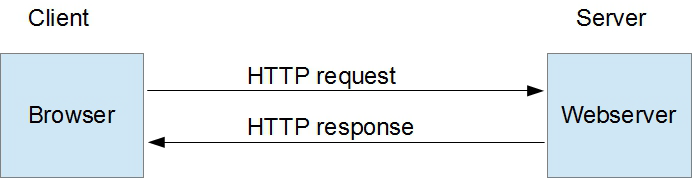
\includegraphics[width=12cm]{images/HTTPZustand0.png}
    \caption{HTTP zustandslos}
    \label{HTTPZustandslos}
    \end{center}
\end{figure}\\
Die einzige Möglichkeit einen Zustand an den Client zu übergeben ist, diesen per weiteren Requests mitzuschicken. Die Zustände werde mit einem Cookie oder einem "`Hidden field"' erfasst.
\begin{figure}[ht]
    \begin{center}
    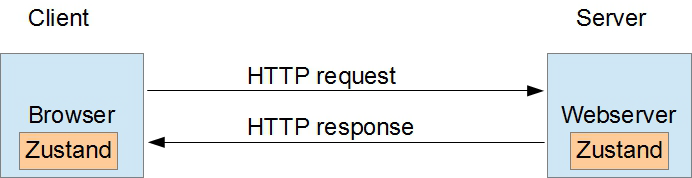
\includegraphics[width=12cm]{images/HTTPZustand1.png}
    \caption{HTTP Zustand per Request (hidden field)}
    \label{HTTPZustand}
    \end{center}
\end{figure}
\paragraph*{Cookies}Cookies sind kurze Textdaten, welche vom Server als Header an den Browser übermittelt werden und von diesem ebenso als Header bei requests wieder mitgesendet werden. Cookies werden vom Browser verwaltet. Die meistgenutzte Möglichkeit ist es, ein Cookie zu setzen. Jedoch dürfen auch Cookies nicht client-seitig angepasst werden können!
\begin{figure}[ht]
    \begin{center}
    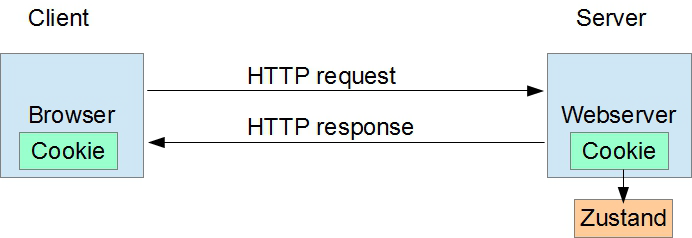
\includegraphics[width=12cm]{images/HTTPCookie.png}
    \caption{Einsatz eines Cookies}
    \label{HTTPCookie}
    \end{center}
\end{figure}
\paragraph*{Cookie Eigenschaften}Die Eigenschaften von Cookies sind:
\begin{itemize}[noitemsep,topsep=0pt,leftmargin=*]
    \item \textbf{Persistent} (mit Ablaufdatum) oder \textbf{Session-Cookie} (ohne Ablaufdatum)
    \item \textbf{Secure} (wird nur über HTTPS übertragen)
    \item \textbf{HTTP Only} (darf nur von HTTP gelesen werden)
    \item \textbf{Same Site} (wird nicht bei Cross-Domain-Aurfrufen mitgesendet, z.B. `embedded' Link, Image)
\end{itemize}

\subsection*{Sie wissen was eine Session ist und welche Eigenschaften einer Session bei welchen Angriffen wichtig sind bzw wie sie gegen gewisse Angriffe Schutz bieten}
\paragraph*{Session} Eine Session ist der Zeitraum, in dem ein Client eine stehende Verbindung mit einem Server hat; vom Login bis zum Logout. Der Server vergibt dem Client eine eindeutige Session-ID. Die Sitzungsdaten (z.B. Warenkorb) werden im Server gespeichert. Bei jedem Request gibt der Client seine Session-ID mit, damit der Server beim Response die zugehörigen Daten dieser ID übermitteln kann. Es gibt auch Sessions ohne stehende Verbindung (ohne Login). Dies wird zu Statistikzwecken verwendet, beispielsweise um die Bewegung des Besuchers auf der Website zu verfolgen. Oder aber auch um einen Warenkorb ohne Login verwenden zu können.
\paragraph*{Schwaches Session-Management:} Was ist das?
\begin{itemize}[noitemsep,topsep=0pt,leftmargin=*]
    \item der Sessionwert ist vorhersagbar
    \item der Sessionwert kann vom Client gesetzt werden
    \item die Cookie-Attribute `Secure', `HttpOnly' oder `Same Site' sind nicht gesetzt
    \item Cookie-Domain oder -Pfad sind nicht so eingeschränkt wie möglich
    \item die Session wird bei einem Logout nicht invalidiert
    \item die Session hat kein server-seitiges Timeout (Inaktivitäts- und absolutes Timeout)
\end{itemize}
\subsection*{Sie kennen sicherheitsrelevante Header}
\paragraph*{TODO}
\subsection*{Sie verstehen wie ein Cross-Site-Request-Forgery-Angriff abläuft und wie man sich dagegen schützen kann}
\paragraph*{TODO}


\section{Angriffe auf Protokollebene}
\subsection*{Sie kennen die Grundbegriffe der Anwendungssicherheit}
\paragraph*{TODO}
\subsection*{Sie kennen Beispiele von Angriffen auf verschiedenen Ebenen des Protokollstacks und wissen was diese bewirken}
\paragraph*{TODO}
\subsection*{Sie verstehen wie ein Cross-Site-Scripting/SQL-injection/Social-Engineering-Angriff abläuft und wie man sich dagegen schützen kann}
\paragraph*{TODO}



\part{Management (SW~07-09)}
\section{Standards \& Frameworks, ISMS}
\subsection*{Sie wissen, was ein ISMS ist und wie man damit umgeht}
\paragraph*{TODO}
\subsection*{Sie kennen die wichtigsten Standards der Informationssicherheit}
\paragraph*{TODO}
\subsection*{Sie finden sich in den Standards ISO 27001 und 27002 zurecht}
\paragraph*{TODO}
\subsection*{Sie verstehen die Grundzüge der BSI-Standards (BSI=Bundesamt für Sicherheit in der Informationstechnik, Deutschland)}
\paragraph*{TODO}
\subsection*{Sie kennen die Struktur und Grundziele des NIST CyberSecurityFrameworks}
\paragraph*{TODO}


\section{Risiko-Management und IT-Grundschutz}
\subsection*{Das Risikoanalyse-Verfahren verstehen}
\paragraph*{TODO}
\subsection*{Die Unterschiede zum Grundschutzverfahren kennen}
\paragraph*{TODO}
\subsection*{Eine einfache Risikoanalyse durchführen können}
\paragraph*{TODO}
\subsection*{Sie verstehen die Idee, die Ziele und die Konzepte des IT-Grundschutz-Vorgehens}
\paragraph*{TODO}
\subsection*{Sie kennen den Aufbau der IT-Grundschutz-Kataloge und deren Anwendungsweise}
\paragraph*{TODO}
\subsection*{Sie können die Teilschritte zum Aufbau eines Sicherheitskonzeptes nach IT-Grundschutz durchführen, kombinierte Risikoanalyse}
\paragraph*{TODO}


\section{Awarness}
\subsection*{Sie verstehen die Wichtigkeit der \flqq Awareness \frqq}
\paragraph*{TODO}
\subsection*{Sie kennen verschiedene Prozesse und Vorgehensweisenfür die Initiierung, Durchführung und Erfolgsprüfung einer Awareness-Kampagne und können diese anwenden}
\paragraph*{TODO}
\subsection*{Sie kennen die relevanten Erfolgsfaktorender Mitarbeiter-Sensibilisierung und -Schulung und können diese in einer Kampagne umsetzen}
\paragraph*{TODO}



\part{Access Control (SW~10)}
\section{Access Control}
\subsection*{Sie kennen verschiedene Arten der Authentisierung, wissen wie diese technisch ablaufen und was deren Vor- und Nachteile sind}
\paragraph*{TODO}
\subsection*{Sie wissen wie verschiedene Authentisierungstoken technisch funktionieren, was deren Vor- und Nachteile sind und wie sie beim Login oder bei der Transaktionsbestätigung im e-Banking eingesetzt werden}
\paragraph*{TODO}
\subsection*{Sie wissen was Authentisierung, Autorisierung ist, warum diese wichtig sind und wie Angriffe darauf ablaufen}
\paragraph*{TODO}


\part{Multi-Party-Computation (SW~11)}
\subsection*{Sie kennen einfache Beispiele von verteilten sicheren Berechnungen und verstehen wie die entsprechenden Protokolle ablaufen}
\paragraph*{TODO}
\subsection*{Sie kennen Arten von Sicherheit von verteilten sicheren Berechnungen und wie diese angegriffen werden können}
\paragraph*{TODO}
\subsection*{Sie wissen welche Eigenschaften elektronisches Geld ausmachen und kennen die technischen Grundlagen von Bitcoin}
\paragraph*{TODO}


\section{Cryptographic Protocols}
\section{Secret Sharing}
\section{Zero Knowledge Proof}
\subsection*{Sie wissen was Zero-Knowledge-Proofs sind und wie diese ablaufen}
\paragraph*{TODO}



\part{Quantum (SW~12)}
\subsection*{Sie wissen was ein Quantencomputer ist und was ihn von einem "`klassischen"' Computer unterscheidet}
\paragraph*{TODO}
\subsection*{Sie verstehen welchen Einfluss die Existenz eines Quantencomputers auf die Kryptographie hat}
\paragraph*{TODO}
\subsection*{Sie verstehen wie Quantenschlüsselaustausch funktionert}
\paragraph*{TODO}


\section{Quantum Computing and Quantum Cryptography}
\part{WAF, Federations (SW~13)}
\section{Firewalls}
\subsection*{Sie wissen was die Aufgaben einer Firewall sind}
\paragraph*{TODO}
\subsection*{Sie verstehen die Funktionsweise einer WAF und wie sie eine Webanwendung vor Angriffen schützen kann}
\paragraph*{TODO}


\section{Federations}
\subsection*{Sie verstehen wie Authentisierung mit Identity Federation abläuft, was die Voraussetzungen dafür sind und was die Vor- und Nachteile von Federations sind}
\paragraph*{TODO}



\part{Talks (SW~14)}
\section{Malware}
\subsection*{Sie verstehen, welche Arten von Malware es gibt, welche Massnahmen gegen Malware sinnvoll sind und wie diese wirken}
\paragraph*{TODO}

\section{WAF}
\subsection*{Sie verstehen wo Machine-Learning in einer WAF eingesetzt werden kann und was einene Machine-Learning-Ansatz vom "`herkömmlichen"' Einsatz einer WAF unterscheidet}
\paragraph*{TODO}
\subsection*{Sie kennen Beispiele von Angriffen, welche mittels Machine-Learning auf einer WAF erkannt werden konnten}
\paragraph*{TODO}
\end{document}